\documentclass[a4paper,12pt]{article}
\usepackage[utf8]{inputenc}
\usepackage{listings}
\usepackage{color}
\usepackage[hidelinks]{hyperref}
\usepackage{geometry}
\geometry{margin=1in}
\usepackage{graphicx}
\usepackage[style=acmnumeric,backend=biber]{biblatex}
\addbibresource{references.bib}

\title{Luna's Library System \\
\vspace{0.5em}
\large Documentation and Code Overview}
\author{Angel E Luna}
\date{\today}

\definecolor{codegray}{rgb}{0.5,0.5,0.5}
\definecolor{codepurple}{rgb}{0.58,0,0.82}
\definecolor{backcolour}{rgb}{0.95,0.95,0.92}

\lstdefinestyle{mystyle}{
    backgroundcolor=\color{backcolour},   
    commentstyle=\color{codegray},
    keywordstyle=\color{blue},
    numberstyle=\tiny\color{codegray},
    stringstyle=\color{codepurple},
    basicstyle=\ttfamily\footnotesize,
    breaklines=true,
    captionpos=b,
    keepspaces=true,
    numbers=left,
    numbersep=5pt,
    showspaces=false,
    showstringspaces=false,
    showtabs=false,
    tabsize=2
}

\lstset{style=mystyle}

\newcommand{\bibliofont}{\normalfont}

\begin{document}

\maketitle

\tableofcontents

\section{Introduction}

Luna's Library System is a console-based application developed in C++ that simulates the core functionalities of a digital library. The system allows users to register, log in, borrow and return various types of library items such as books, theses, and magazines, and to view their borrowing history. All user and library data are stored persistently using CSV files, ensuring that information is retained between sessions.

The project was designed to provide a practical demonstration of object-oriented programming principles, file handling, and menu-driven user interfaces in C++. By tackling common challenges found in real-world library management—such as user authentication, data consistency, and resource tracking—this system serves as both a learning tool and a foundation for further development. The modular structure of the code makes it easy to extend with new features or adapt to different requirements.

This documentation provides a comprehensive overview of the system's design, functionality, and usage, along with guidelines for future development and extension.

\section{Project Motivation and Rationale}

The decision to develop Luna's Library System was driven by several key factors:

\begin{itemize}
    \item \textbf{Practical Application of C++ Concepts:} This project provides a comprehensive exercise in object-oriented programming, file I/O, and data structures, all of which are fundamental to mastering C++. By implementing a real-world system, the project bridges the gap between theoretical knowledge and practical skills.
    \item \textbf{Relevance to Everyday Needs:} Library management is a classic problem that remains relevant in both educational and professional contexts. Designing a digital library system simulates challenges faced in real information systems, such as user authentication, data persistence, and resource management.
    \item \textbf{Scalability and Extensibility:} The project was chosen for its potential to be extended with new features, such as additional file types, advanced search, or even a graphical interface. This makes it an ideal foundation for future learning or collaborative development.
    \item \textbf{Personal Interest and Challenge:} Building a library system is both intellectually stimulating and rewarding. It requires careful planning, attention to detail, and creative problem-solving, making it an ideal project for honing software development skills.
\end{itemize}

\section{Project Structure}
\begin{itemize}
    \item \texttt{main.cpp} -- Main program logic and menu handling
    \item \texttt{bibliofiles.hpp} -- Base and derived classes for library items (Book, Thesis, Magazine)
    \item \texttt{user.csv} -- Stores user data
    \item \texttt{books.csv}, \texttt{thesis.csv}, \texttt{mags.csv} -- Store library items
\end{itemize}

\section{Main Features}
\begin{itemize}
    \item User registration and login
    \item Borrowing and returning files
    \item Viewing file information and fragments
    \item Persistent storage using CSV files
    \item User history tracking
\end{itemize}

\section{Class Overview}

\subsection{BiblioFiles and Derived Classes}
\begin{lstlisting}[language=C++, caption={BiblioFiles Base Class}]
class BiblioFiles {
protected:
    std::string idfile, title, author, filetype, fragment;
    int publicationyear;
    bool availability;
public:
    // Methods for getting info, showing fragments, etc.
};
\end{lstlisting}

\textbf{Book}, \textbf{Thesis}, and \textbf{Magazine} inherit from \texttt{BiblioFiles} and add specific fields and methods.

\subsection{User Class}
\begin{lstlisting}[language=C++, caption={User Class}]
class User {
protected:
    std::string history;
    std::string name, password;
    std::string borrowedfiles;
public:
    void borrowfile(BiblioFiles* file);
    void returnfile(BiblioFiles* file);
    // Other user-related methods
};
\end{lstlisting}

\section{Program Flow}

\subsection{Startup}
\begin{enumerate}
    \item Loads user data from \texttt{user.csv}.
    \item Displays the main menu: Login, Register, Exit.
\end{enumerate}

\subsection{Login and Registration}
\begin{itemize}
    \item On login, verifies username and password.
    \item On registration, checks for unique username and appends new user to \texttt{user.csv}.
\end{itemize}

\subsection{Library Data Loading}
After successful login, the program loads library data from \texttt{books.csv}, \texttt{thesis.csv}, and \texttt{mags.csv}.

\subsection{Main Application Loop}
\begin{enumerate}
    \item Shows user menu: View files, Search, Borrow, Return, History, User Settings, Exit.
    \item Handles user actions with nested menus and input validation.
    \item Updates user and library data in memory and in CSV files.
\end{enumerate}

\section{File Operations}
\begin{itemize}
    \item Reading: Uses \texttt{std::ifstream} and \texttt{std::getline} to load data.
    \item Writing: Uses \texttt{std::ofstream} (with \texttt{std::ios::app} for appending or \texttt{std::ios::trunc} for overwriting).
    \item Updates: Reads all lines, modifies in memory, then rewrites the file.
\end{itemize}

\section{Example: Borrowing a File}
\begin{lstlisting}[language=C++]
void User::borrowfile(BiblioFiles* file) {
    if (!history.empty()) history += ";";
    history += file->getidfile();
    // Update user.csv with new borrowed file and history
}
\end{lstlisting}

\section{Error Handling}
\begin{itemize}
    \item The program checks for file open errors and invalid data.
    \item On fatal errors (e.g., missing CSV files), the program prints an error and exits.
    \item Input is validated at each menu to prevent invalid actions.
\end{itemize}

\section{Data Consistency}
The system reads the entire CSV file into memory on startup and writes back any changes immediately. This ensures that all user and library data is consistent and up-to-date.

\section{Object-Oriented Programming Concepts Used}

\subsection{Inheritance}
Inheritance allows a class to use the properties and methods of another class. This promotes code reuse and logical hierarchy. A child class inherits from a parent class and can also add its own functionality.

\subsection{Access Modifiers}
Access modifiers control the visibility of class members:
\begin{itemize}
    \item \textbf{public}: Accessible from anywhere.
    \item \textbf{private}: Accessible only within the same class.
    \item \textbf{protected}: Accessible within the class and its subclasses.
\end{itemize}
They help with encapsulation and data protection.

\subsection{Method Overloading and Overriding}
\textbf{Overloading:} When a class has multiple methods with the same name but different parameter lists. This is resolved at compile time.

\textbf{Overriding:} When a subclass redefines a method from its parent class to provide specific behavior. This is resolved at runtime, usually using \texttt{virtual} in languages like C++.

\subsection{Polymorphism}
Polymorphism allows the same interface to be used for different data types or behaviors. It enables flexibility and code reuse. There are two main types:
\begin{itemize}
    \item \textbf{Compile-time polymorphism} (e.g., method overloading)
    \item \textbf{Runtime polymorphism} (e.g., method overriding using base class pointers or references)
\end{itemize}

\subsection{Abstract Classes}
An abstract class cannot be instantiated on its own. It often contains one or more pure virtual functions, which means any subclass must implement those functions. It serves as a blueprint for other classes.

\subsection{Operator Overloading}
Operator overloading lets you redefine the behavior of standard operators (like \texttt{+}, \texttt{-}, \texttt{==}) when they are used with objects of your own classes. This makes your custom types easier to use and understand.

\section{Future Work and Enhancements}
Potential future enhancements include:
\begin{itemize}
    \item Adding more file types (e.g., audiobooks, videos)
    \item Implementing advanced search and filtering options
    \item Developing a graphical user interface (GUI)
    \item Adding networked multi-user support
    \item Implementing a web-based interface
\end{itemize}

\section{Conclusion}
Luna's Library System is a robust and flexible foundation for understanding and developing library management systems. It covers essential programming concepts and provides a platform for future enhancements and learning.

\section{Program Execution Examples}

This section provides screenshots and sample outputs to illustrate how Luna's Library System appears during execution.

\subsection{Startup and Main Menu}
\begin{figure}[ht!]
    \centering
    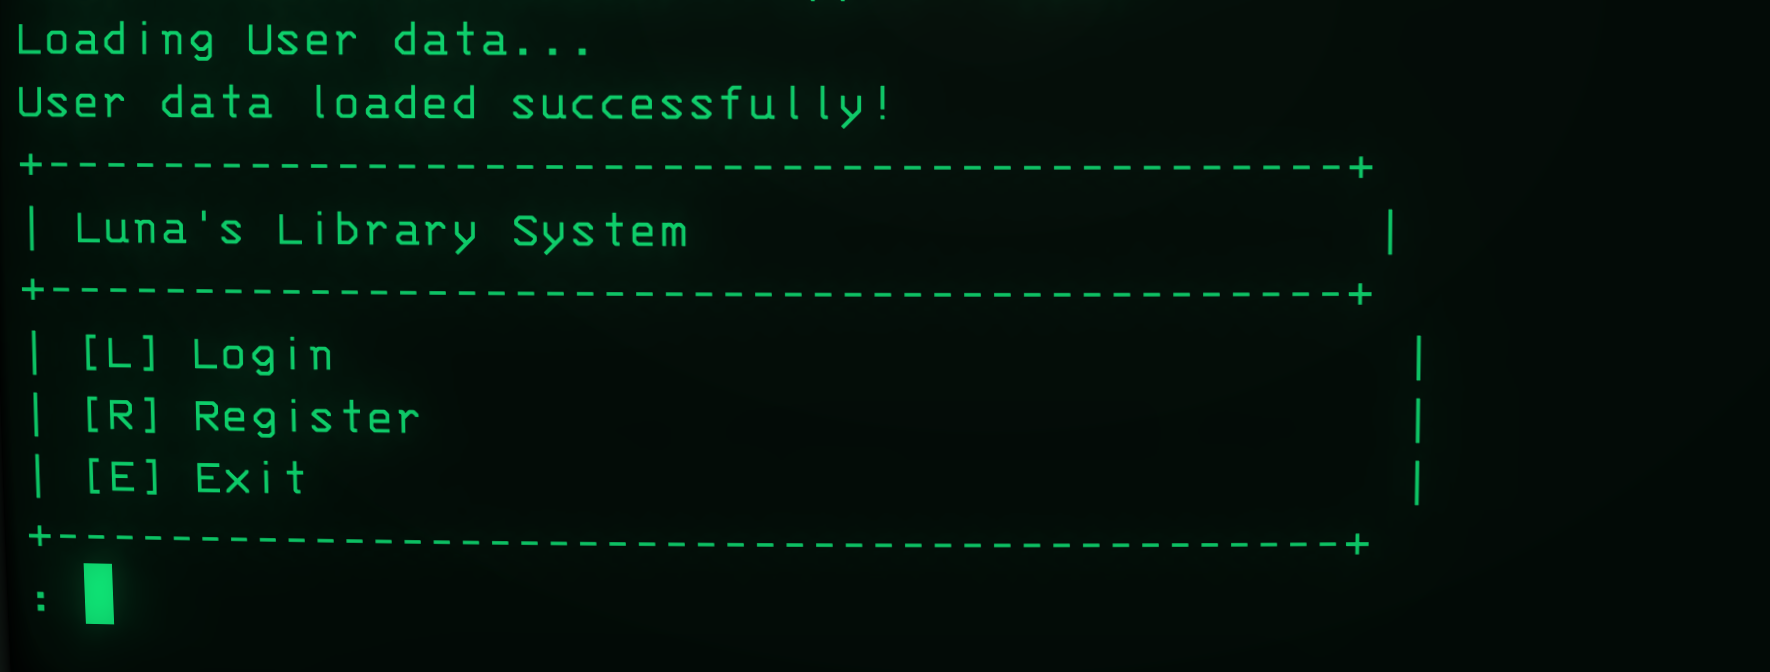
\includegraphics[width=0.8\textwidth]{Screenshot 2025-06-12 at 20.52.09.png}
    \caption{Screenshot 2025-06-12 at 20.52.09.png --- Main menu displayed at program startup.}
\end{figure}

\subsection{User Registration}
\begin{figure}[ht!]
    \centering
    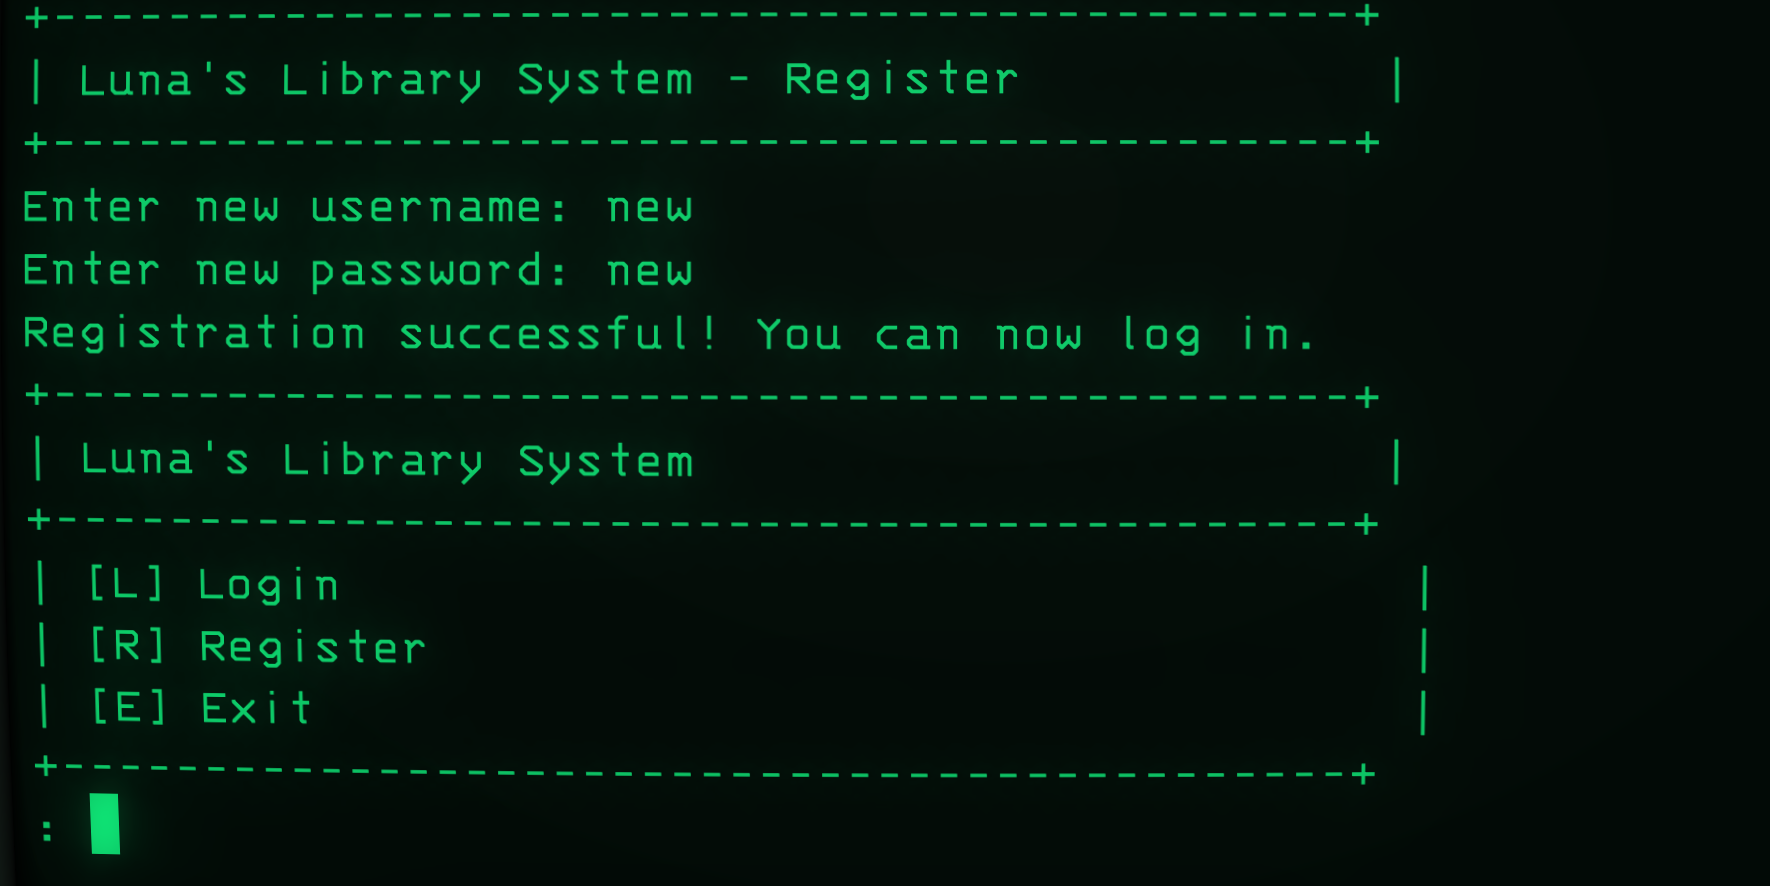
\includegraphics[width=0.8\textwidth]{Screenshot 2025-06-12 at 20.52.34.png}
    \caption{Screenshot 2025-06-12 at 20.52.34.png --- User registration process.}
\end{figure}

\subsection{Login}
\begin{figure}[ht!]
    \centering
    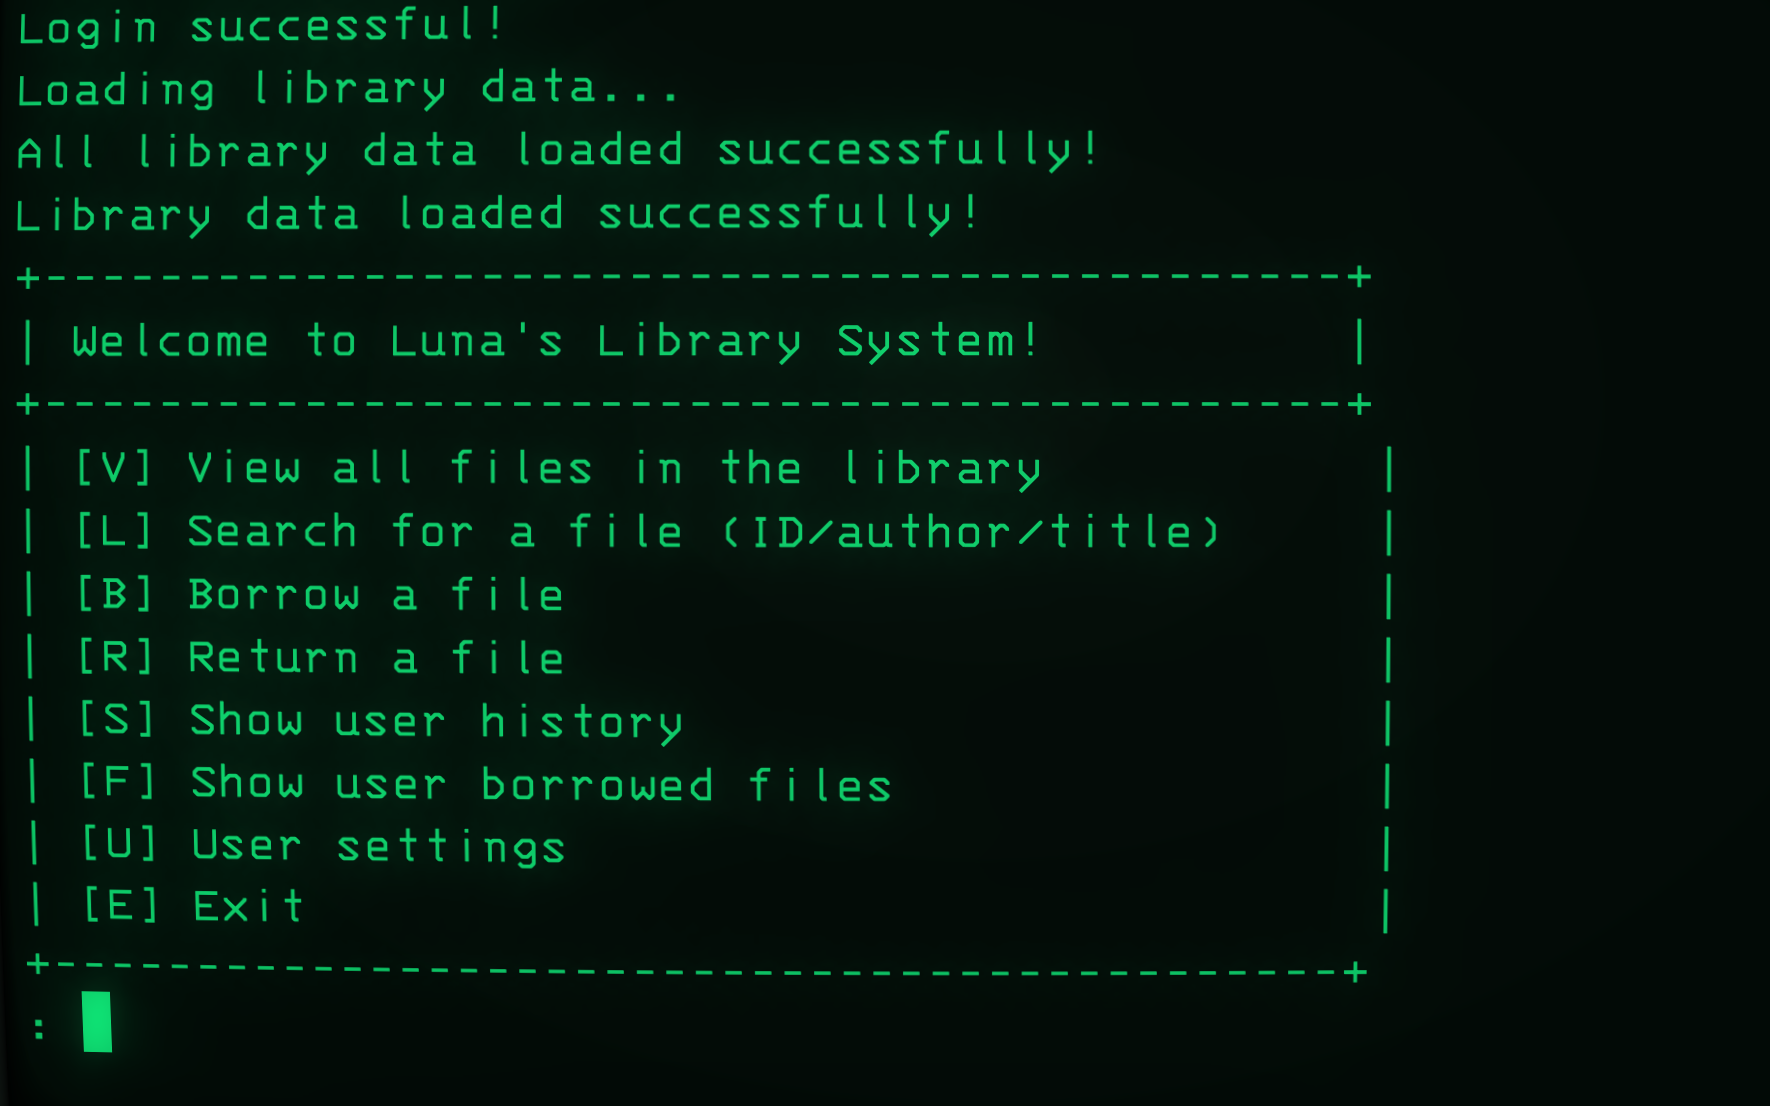
\includegraphics[width=0.8\textwidth]{Screenshot 2025-06-12 at 20.53.00.png}
    \caption{Screenshot 2025-06-12 at 20.53.00.png --- User login prompt.}
\end{figure}

\subsection{Viewing Library Files}
\begin{figure}[ht!]
    \centering
    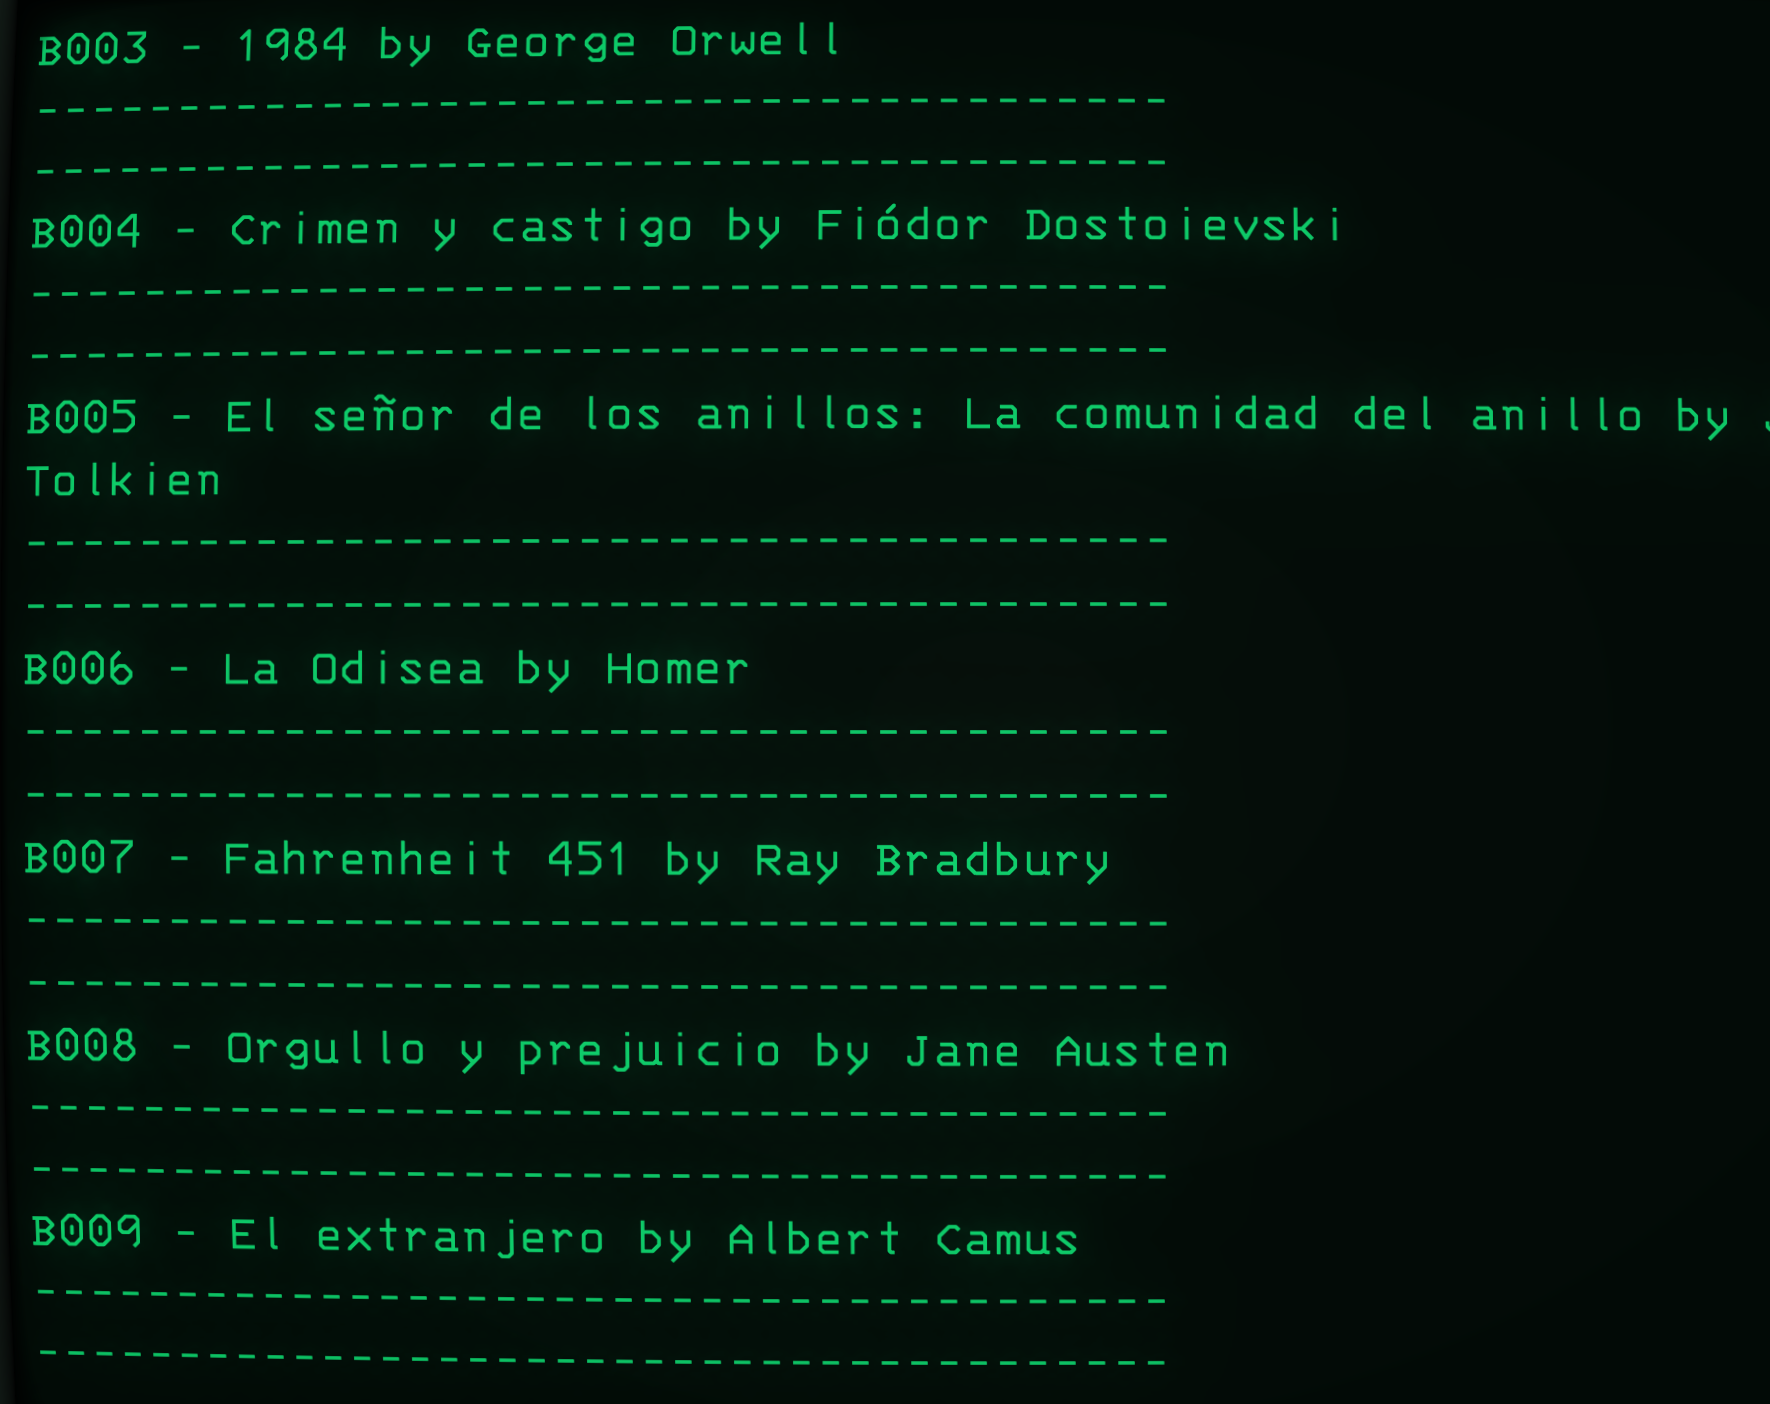
\includegraphics[width=0.8\textwidth]{Screenshot 2025-06-12 at 20.53.23.png}
    \caption{Screenshot 2025-06-12 at 20.53.23.png --- Viewing all files in the library.}
\end{figure}

\subsection{Borrowing a File}
\begin{figure}[ht!]
    \centering
    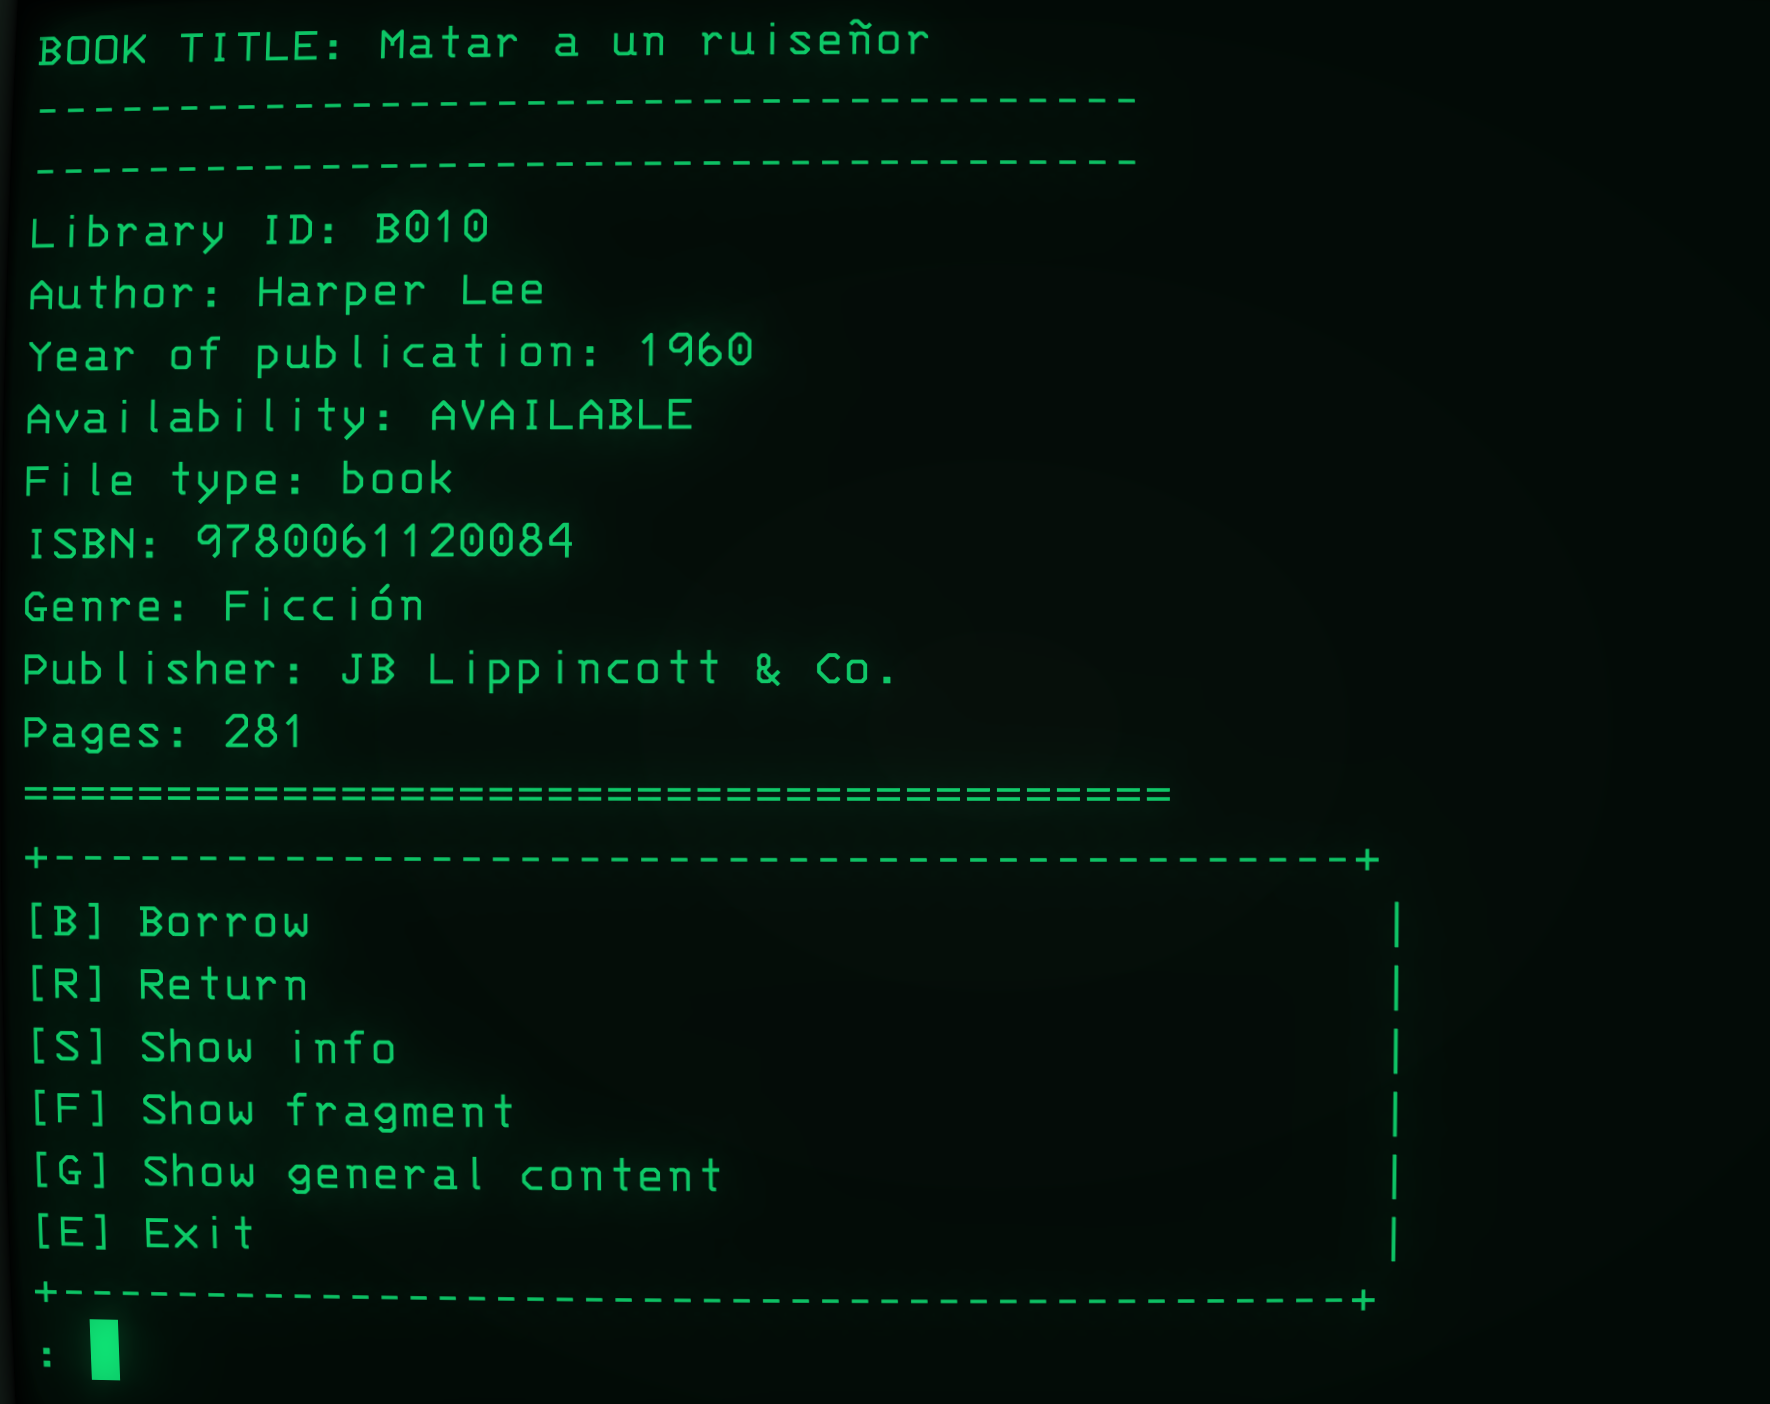
\includegraphics[width=0.8\textwidth]{Screenshot 2025-06-12 at 20.53.52.png}
    \caption{Screenshot 2025-06-12 at 20.53.52.png --- Borrowing a file from the library.}
\end{figure}

\subsection{Returning a File}
\begin{figure}[ht!]
    \centering
    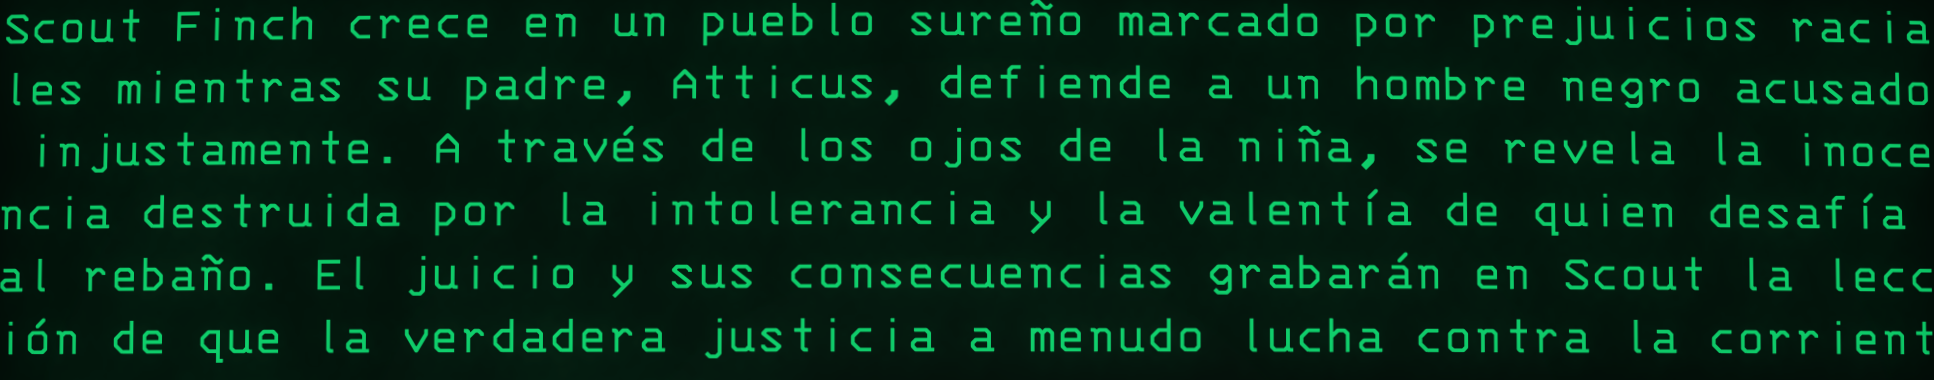
\includegraphics[width=0.8\textwidth]{Screenshot 2025-06-12 at 20.54.10.png}
    \caption{Screenshot 2025-06-12 at 20.54.10.png --- Returning a borrowed file.}
\end{figure}

\subsection{User History}
\begin{figure}[ht!]
    \centering
    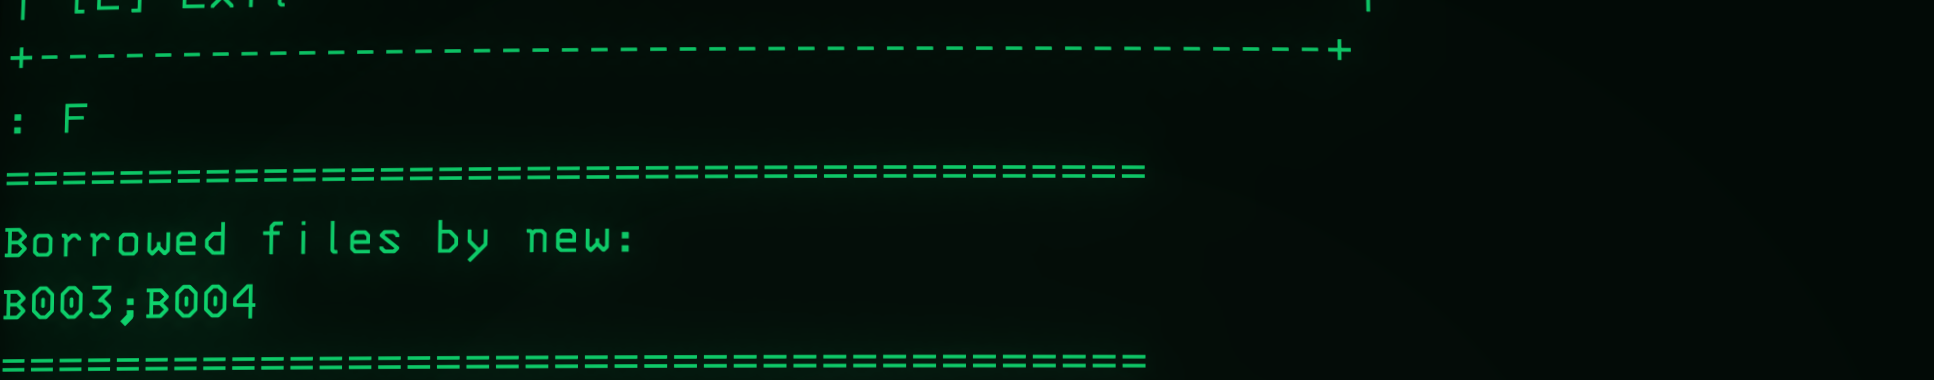
\includegraphics[width=0.8\textwidth]{Screenshot 2025-06-12 at 20.55.30.png}
    \caption{Screenshot 2025-06-12 at 20.55.30.png --- Viewing user borrowing history.}
\end{figure}

\subsection{User Settings}
\begin{figure}[ht!]
    \centering
    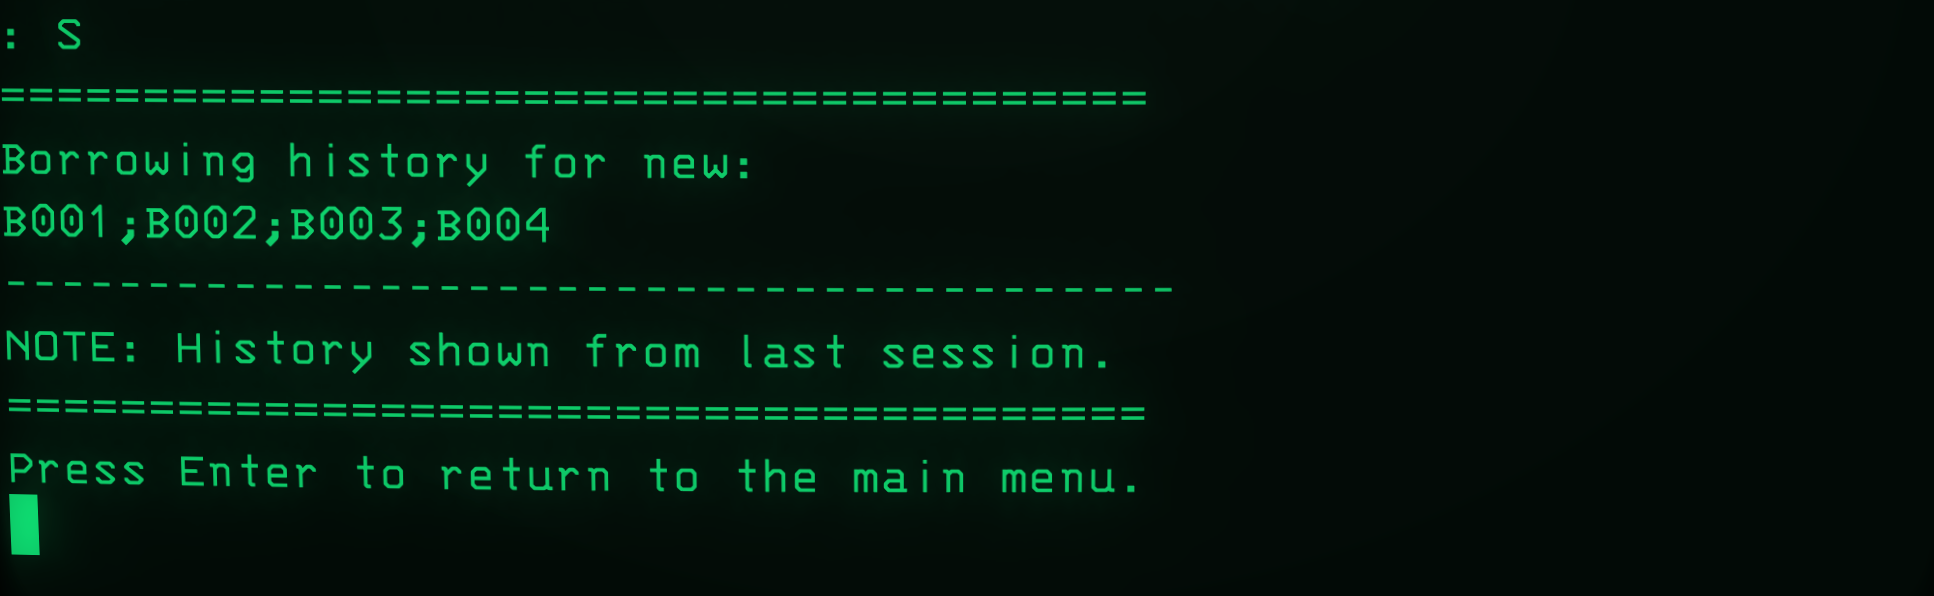
\includegraphics[width=0.8\textwidth]{Screenshot 2025-06-12 at 20.55.55.png}
    \caption{Screenshot 2025-06-12 at 20.55.55.png --- User settings menu.}
\end{figure}

\subsection{Exiting the Program}
\begin{figure}[ht!]
    \centering
    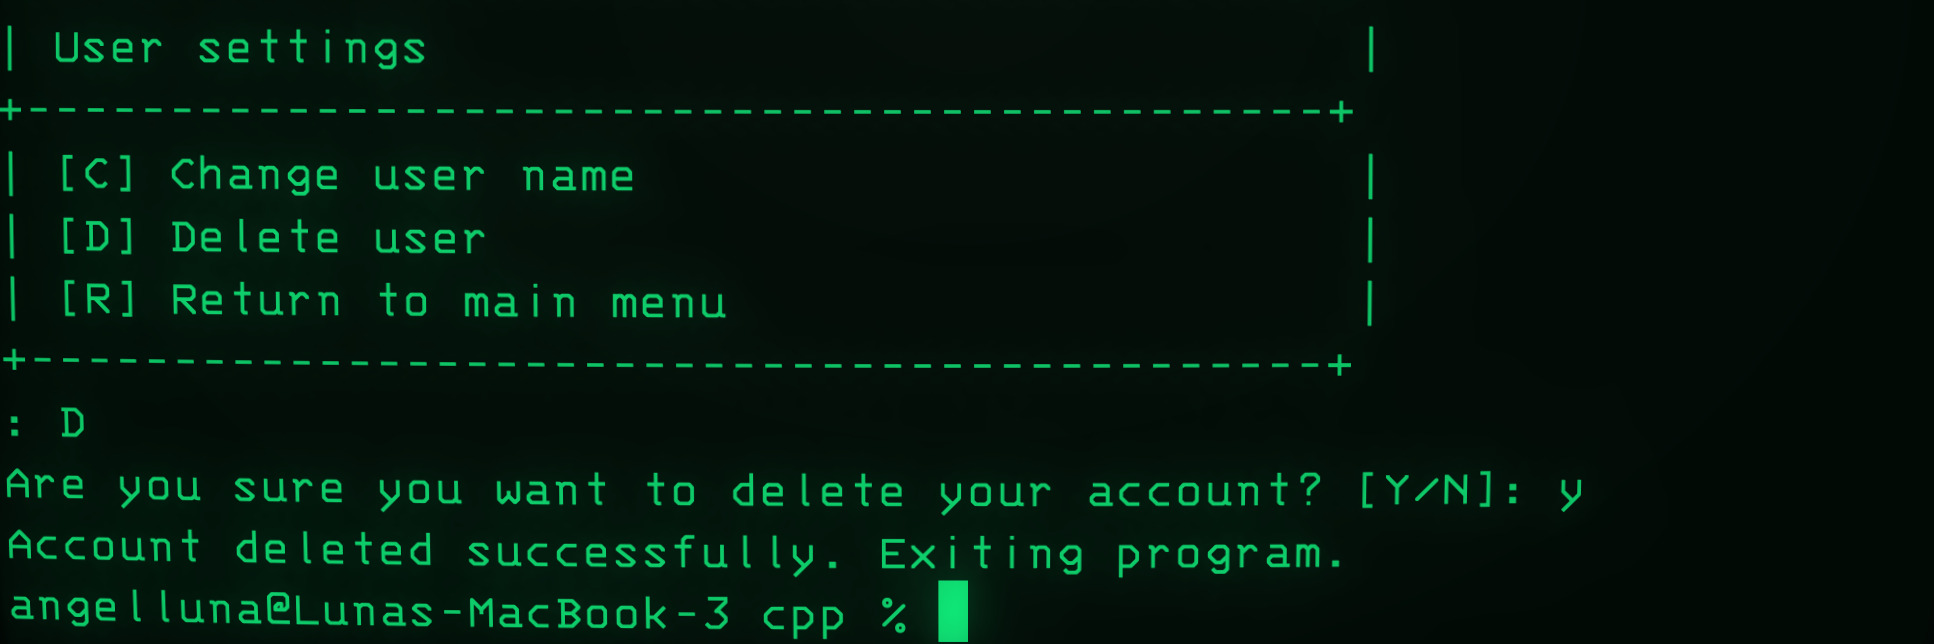
\includegraphics[width=0.8\textwidth]{Screenshot 2025-06-12 at 20.56.20.png}
    \caption{Screenshot 2025-06-12 at 20.56.20.png --- Exiting the program.}
\end{figure}

% Add more figures as needed for other features

\clearpage

\nocite{*}
\printbibliography

\end{document}